% Chapter Template

\chapter{Powering circuit design} % Main chapter title
\label{Chapter4}
In this chapter, we will present some of the engineering challenges faced during the \textbf{design of a power circuit} for our flexible voice coil actuator.
We will mostly describe an ideal circuit as we will later demonstrate that running this actuator would require very \textbf{advanced analog circuitry}, comprised of \textbf{high-cost components}.
Most of the tests we will present have been done using a \textbf{laboratory bench signal generator and amplifier}.


%----------------------------------------------------------------------------------------
%	SECTION 1
%----------------------------------------------------------------------------------------
\section{Power Circuit Block diagram}

%----------------------------------------------------------------------------------------
%	SECTION 2
%----------------------------------------------------------------------------------------
\section{Controller}
The controller in this application has to be a \textbf{signal generator} that can produce a waveform that can be amplified and sent to the coil.
The controller we used for testing is an ESP32 microcontroller.
We chose this controller as the first test hardware for its \textbf{simplicity of programming} and its \textbf{integrated DAC}.

% -- Subsection 4.1
\subsection{ESP32 DAC Characteristics}
The DAC included in the ESP32 is a pretty basic one but as a first test, it is enough.
The DAC has a resolution of \textbf{8 bits}, and it can output a voltage between \textbf{0} and \textbf{3.3V} with a maximum current output of \textbf{12mA}.

\subsection{ESP32 waveform generator}
Using a simple program the ESP32 can be used as a pretty capable waveform generator.
The software we used is the \textbf{ESP32 Signal Generator} from \textbf{\href{https://corz.org}{corz.org}} \cite{corz_signal_gen}.
This software allows the user to generate the following waveforms:
\begin{itemize}
    \item Sine wave from 16Hz to 500kHz
    \item Square wave from 1Hz to 40MHz
    \item Triangle wave from 153Hz to 150kHz 
    \item Sawtooth wave from 153Hz to 150kHz
\end{itemize}

\begin{samepage}
    Between these ranges of frequencies, the generated waveforms are pretty accurate.
    \nopagebreak

    \begin{figure}[H]
        \centering
        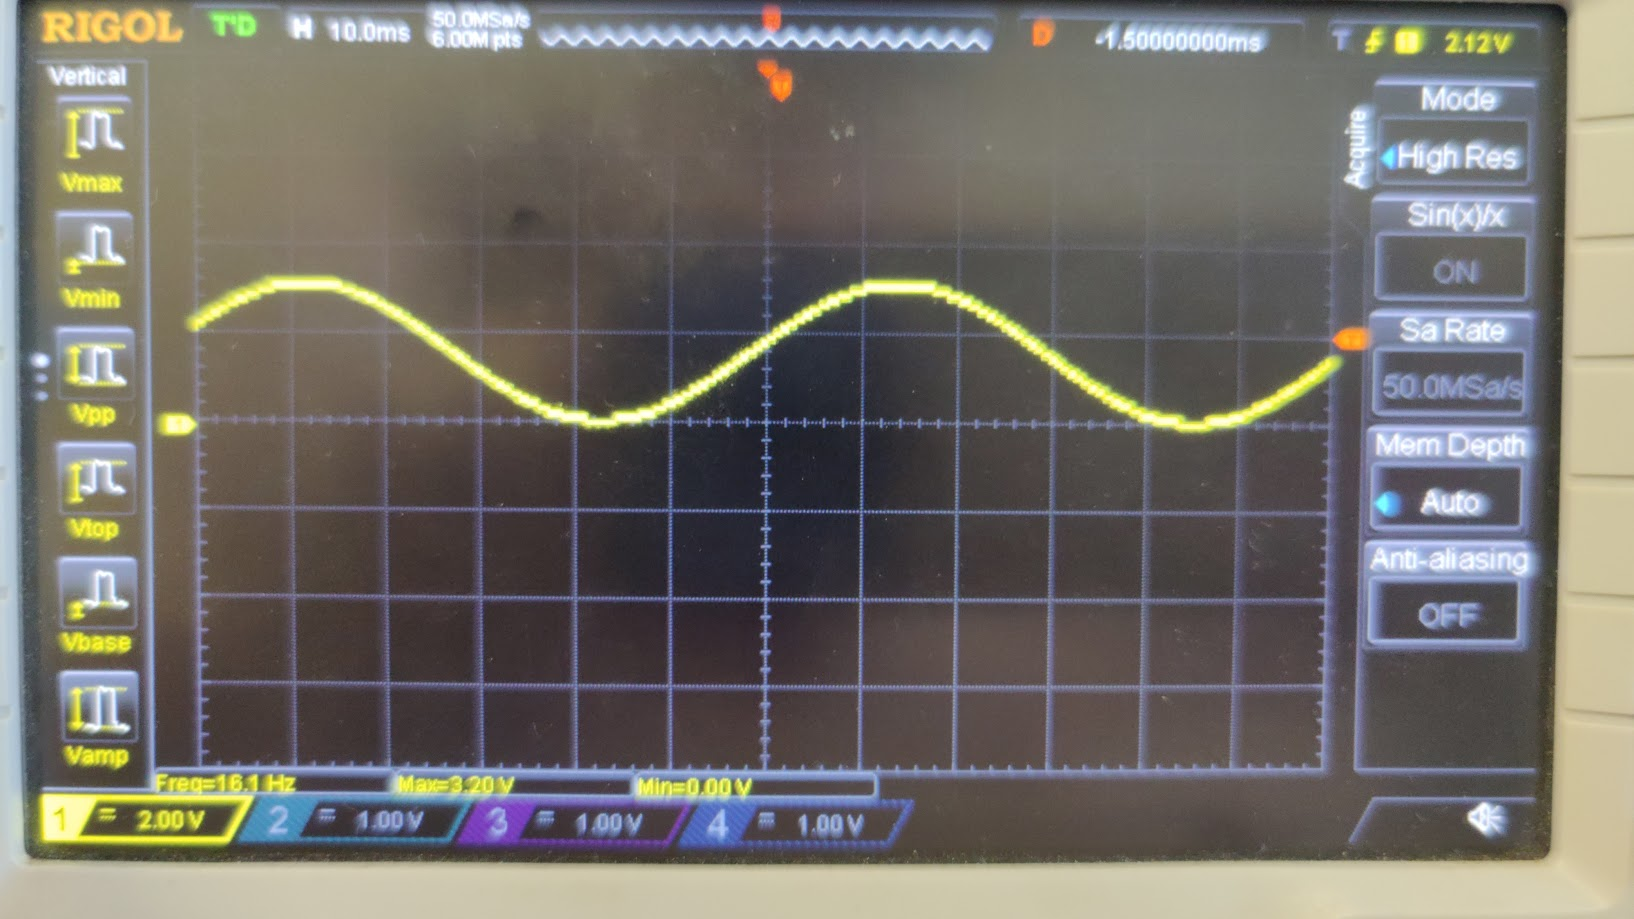
\includegraphics[width=0.9\linewidth]{Chapters/Chapter4/Figures/16Hz_signal_gen.jpg}
        \caption[ESP32 DAC in action]{ESP32 16Hz Sine wave generated by the ESP32 Signal Generator software.}
        \label{fig:16Hz_signal_gen}
    \end{figure}
\end{samepage}

\pagebreak

% \subsubsection{Esp32 DAC limitations}

% \subsubsection{Esp32 DAC Noise}


%----------------------------------------------------------------------------------------
%	SECTION 3
%----------------------------------------------------------------------------------------
\section{Signal Conditioning Circuit}
\label{Signal_Conditioning_Circuit}
We know that the controller DAC \textbf{outputs a voltage} between \textbf{0} and \textbf{3.3V}, the power stage has a \textbf{gain of 10}, and that to drive Flexar's coils, at their rated \textbf{maximum power of 0.8W}, we need to provide a voltage of about \textbf{6V} at a current of \textbf{0.2A}. \\
A very simple solution is to implement a \textbf{variable voltage divider} to adjust the amplitude of the signal coming from the DAC.

\begin{samepage}
    We chose a \textbf{maximum dividing factor of 10} to match the power stage gain.
    \nopagebreak

    \begin{figure}[H]
        \centering
        \resizebox{.5\linewidth}{!}{\begin{circuitikz}[american]
    \draw (0,0) node[ground]{} to[sV, l=$V_{DAC}$] (0,3) to[vR, l=$R_1$] (3,3) to[R, l=$R_2$] (3,0) node[ground]{};
    \draw (3,3) to[short, -o] (4,3) node[right]{$V_{out}$};
\end{circuitikz}}
        \caption{Signal conditioning circuit.}
        \label{fig:cond_circuit}
    \end{figure}
    \nopagebreak

    Where:
    \nopagebreak

    \begin{itemize}
        \item $V_{DAC}$ is the voltage coming from the controller DAC [0,3.3]V.
        \item $R_1$ is a 100$k\Omega$ potentiometer to adjust the amplitude of the signal.
        \item $R_2$ is a 10$k\Omega$ resistor to set the maximum amplitude of the signal.
        \item $V_{out}$ is the output voltage of the conditioning circuit [0, 0.33]V.
    \end{itemize}
\end{samepage}

The output voltage of the conditioning circuit is given by the following formula:
\begin{equation}
    V_{out} = V_{DAC} \cdot \frac{R_1}{R_1 + R_2}
\end{equation}

The values of $R_1$ and $R_2$ have been chosen to be 100$k\Omega$ and 10$k\Omega$ respectively, as they are standard values, provide a good range of adjustment for the amplitude of the signal, and their order is \textbf{big enough} to work with the provided DAC current of 12mA.

%----------------------------------------------------------------------------------------
%	SECTION 4
%----------------------------------------------------------------------------------------
\section{Amplifier circuit}
The online architecture operates in real-time. It processes the input data from the camera and produces as output the satellite pose estimation.

After being pre-processed, the image captured from the camera is passed to the \textit{Landmark regression} module. The latter predicts the 2D location \{\(\textbf{z}_i\)\} of the 9 landmarks along with the visibility coefficient \{\(v_i\)\} for each of them. The \textit{Landmark Mapping} module then uses these data to compute the 3D position of each landmark with respect to the camera frame. The final 6DOF pose of the satellite is then computed from the CPD module. Figure \textbf{\ref{fig:Online Pipeline}} shows the online pipeline of the implemented methodology.
\begin{figure}[H]
    \centering
    \includegraphics[scale=0.6]{Figures/Chapter4/Online Pipeline.png}
    \caption[Online pipeline of the implemented pose estimator.]{Online pipeline of the implemented pose estimator.}
    \label{fig:Online Pipeline}
\end{figure}

% -- Subsection 2.1
\subsection{High Power Operational Amplifiers}
\label{Chapter4/Pre-Processing}
The image captured from the camera is pre-processed in the \textit{Pre-Processing} module. It consists in a bilateral filter, which is a non-linear, edge-preserving smoothing filter that reduces noise while preserving the edges in an image.\\
The mathematical steps behind the bilateral filter involve computing weighted averages of pixel values within a local neighborhood. 
\begin{figure}[th]
    \centering
    \includegraphics[scale=0.32]{Figures/Chapter4/bilateral_filtering.png}
    \caption[Bilateral Filter.]{Bilateral Filter mathematical steps.}
    \label{fig:Bilateral Filter}
\end{figure}

The formula for the bilateral filter operation can be described as follows:

Given an input image \(I(x, y)\) and the filter parameters:
\begin{itemize}
    \item \(d\) (diameter of each pixel's neighborhood)
    \item \(\sigma_c\) (standard deviation of the color space)
    \item \(\sigma_s\) (standard deviation of the spatial space)
\end{itemize}
The filtered output image \(B(x, y)\) can be computed using the following equation for each pixel \((x, y)\):
\begin{equation}
   B(x, y) = \frac{1}{W(x, y)} \sum_{(i, j) \in S} I(i, j) \cdot G_c(I(x, y), I(i, j), \sigma_c) \cdot G_s(x, y, i, j, \sigma_s) 
\end{equation}


Where:
\begin{itemize}
    \item \(S\) is the neighborhood of pixel \((x, y)\), defined by a window of diameter \(d\).
    \item \(G_c\) is the color similarity term, which measures the similarity in color between pixels \((x, y)\) and \((i, j)\) in the color space.
    \item \(G_s\) is the spatial similarity term, which measures the spatial proximity between pixels \((x, y)\) and \((i, j)\).
    \item \(W(x, y)\) is a normalization factor.
\end{itemize}
The \(G_c\) term is defined as a Gaussian function in the color space:
\begin{equation}
    G_c(I(x, y), I(i, j), \sigma_c) = \exp\left(-\frac{\|I(x, y) - I(i, j)\|^2}{2\sigma_c^2}\right)
\end{equation}

The \(G_s\) term is a Gaussian function in the spatial space:
\begin{equation}
    G_s(x, y, i, j, \sigma_s) = \exp\left(-\frac{\|(x, y) - (i, j)\|^2}{2\sigma_s^2}\right)
\end{equation}

\begin{figure}[th]
    \centering
    \includegraphics[scale=0.5]{Figures/Chapter4/Pre-processing.png}
    \caption[Input and pre-processed image.]{On the left the original sample image from the training dataset, on the right the resultant image after the application of the bilaterial filter ($d = 40,\sigma_c = 40,\sigma_s = 200$).}
    \label{fig:Pre-processing}
\end{figure}

The bilateral filter operates by applying these Gaussian weighting functions to compute the weighted average of pixel values within the defined neighborhood, both in color and spatial spaces, resulting in a smoothed image that preserves edges and details. The filter helps reduce noise while keeping the important structures in the image intact.

\subsubsection{Old type of op-amp}
\subsubsection{Power dissipation problems}

% -- Subsection 2.2
\subsection{High Power Voltage Amplifier}
\label{Chapter4/CPD}
As the \textit{Landmark Mapping} module predicts the position of each landmark independently one from the other and so each landmark has its own error over the three axis, the resultant cloud of points is misaligned with respect to the rigid reference position given by the CAD model.\\
In order to estimate the 6DOF pose of the satellite and in the meantime overcome this misalignment problem a mathematical technique is used: Coherent Point Drift.

Two sets of 3D points are present: one is the "target", which represents the 3D position of the landmarks in the camera frame supposing no translation and no rotation, and the other is "source", which is the 3D position of the predicted landmarks.
The "source" point set is only composed by landmarks identified in the image frame (\(v_i = 1\)). It is important to know that the algorithm's performances strongly depend on the number of points in the set so, with the camera approaching the target, some landmarks are cut from the image frame and consequently the pose estimation accuracy reduces.

\begin{figure}[H]
    \centering
    \includegraphics[scale=0.23]{Figures/Chapter4/CPD.png}
    \caption[Iterations of the CPD optimization process.]{Iterations of the CPD optimization process.}
    \label{fig:CPD}
\end{figure}

% %----------------------------------------------------------------------------------------
% %	SECTION 5
% %----------------------------------------------------------------------------------------
% \section{Power Supply}

% %----------------------------------------------------------------------------------------
% %	SECTION 6
% %----------------------------------------------------------------------------------------
% \section{Implementation problems and possible alternatives}

% -- Subsection 5.1
\subsection{Non idealities}
\label{Chapter4/LandmarksSel}
The main problem in the implementation of the \textit{Landmark regression} module (\textbf{\ref{Chapter4/LandReg}}) is the selection of the landmarks.
Selecting meaningful landmarks is a critical first step, requiring a accurate understanding of the satellite's structure. These landmarks must possess distinct characteristics that remain invariant under varying conditions, such as changes in lighting, orientation, or potential occlusions.

The first performed attempt in the selection of the landmarks was composed of 11 landmarks with relevant features in the satellite's structure. Most of those visual features were similar to each others and the resultant heatmap predicted by the CNN for a single landmark was ambiguous among multiple ones. This led to a complicated recognition of the landmark location in the image with complex and heavier algorithms for the 2D position identification.

In both cases the set of landmarks has been selected near the approach target to limit the number of out of frame landmark in closer positions.

\subsubsection{Stability}

\subsubsection{Phase Shift}

\subsubsection{Noise}

% -- Subsection 5.2
\subsection{Polarized signals}

% -- Subsection 5.3
\subsection{Alternative Amplifiers}
\label{Chapter4/DatasetAv}
Another notable challenge stems from the limited size of available datasets. A smaller dataset poses a risk of overfitting, potentially hindering the model's ability to generalize across diverse scenarios. Addressing this issue requires careful consideration of data augmentation techniques, introducing various transformations to enhance the model's adaptability.

The dataset used for training present five different orientations on each axis of the satellite during the whole approaching range. The main limitation given by the used dataset is the lack of combined rotations over multiple axis and a wider range of rotation on single axis.

Even though the \textit{Landmark regression} module training is strictly related to the availability of the images, the \textit{Landmarks Mapping} one is totally independent. The 2D-3D correspondence of landmarks used to train the model requires the only relative position of the landmarks from the CAD Model and the perspective matrix to be performed. This means that a possible further step to expand the dataset is to perform several simulations with rotations over multiple axis to create new wider datasets and improve the model performances.

\subsubsection{Current Amplifiers}

